%Tech Science Press — CMC variant of the MA-SQLGrid manuscript
%=================================================================
\documentclass[cmc,article,submit,moreauthors,pdftex]{Definitions/tsp}
\input{Definitions/package}
\input{Definitions/unicode}

% \usepackage[OT1,OT2,T2A,T2B,T2C,T3,T5,T1]{fontenc}
% \usepackage[russian,english]{babel}
\usepackage[english]{babel}

%=================================================================
% Internal commands: Article information and pagination will be assigned by the Editorial Office
\continuouspages{}
\firstpage{1}
\makeatletter
\setcounter{page}{\@firstpage}
\makeatother
\pubvolume{0}
\issuenum{0}
\elocationid{0}
\articlenumber{0}
\pubyear{2026}
\copyrightyear{2026}
\datereceived{Day Month Year}
\dateaccepted{Day Month Year}
\dateonlinefirst{}
\datepublished{Day Month Year}

%=================================================================
% Full title of the paper (Capitalized)
\Title{MA-SQLGrid: A Multi-Stage Context-Grounding Framework for Text-to-SQL over a Power-Grid Maintenance Database}

% Authors, for the paper (add full first names)
\Author{Bijing Liu\textsuperscript{1,2}, Chenglong Sun\textsuperscript{1,2} and Yong Yang\textsuperscript{1,2,*}}

% Authors, for metadata in PDF
\AuthorNames{Bijing Liu, Chenglong Sun and Yong Yang}

% Affiliations / Addresses
\address{%
\textsuperscript{1}NARI Group Corporation (State Grid Electric Power Research Institute), Nanjing 211106, Jiangsu Province, China

\textsuperscript{2}Beijing Kedong Electric Power Control System Co., Ltd., Beijing 100080, China
}%

% Contact information of the corresponding author
\corres{Corresponding Author: Yong Yang. Email: yangyong1@sgepri.sgcc.com.cn}

% Abstract (Do not use inserted blank lines, i.e. \\)
\abstract{Text-to-SQL in power-grid maintenance requires exact grounding to a fixed schema, canonical values, and an explicit answer contract. This paper presents MA-SQLGrid, a lightweight multi-stage pipeline that selects schema and value context, normalizes domain expressions, infers answer shape, generates SQL, and applies reference-free execution-based validation. On the held-out 180-question split of the synthetic GridDB-Maintenance-v2 v0.1 benchmark, the complete compact, domain-normalized, contract-aware condition increases strict execution accuracy relative to prompting with the full schema and values, from 0.4389 to 0.7000 with \texttt{gpt-5.4-mini} and from 0.3389 to 0.7000 with \texttt{deepseek-chat}. Because these conditions also differ in value normalization and question-specific answer-shape guidance, the comparison does not isolate compactness. Adding validation raises the scores to 0.7278 and 0.7667, respectively; the gain for the primary generator is not statistically significant and is treated as diagnostic. Under the combined order-insensitive and projection-tolerant metric, the full-schema condition outperforms the compact condition for both generators. This reversal shows that the strict advantage depends strongly on projection and ordering conformance, although the combined relaxed metric does not by itself establish the relative row-retrieval capability of the two conditions. Compact prompting reduces the estimated rendered-prompt token count by 63.5\%; provider-reported input tokens fall by 23.4\% on the original serving stack and by 74.7\% on the direct second-model endpoint. Three additional temperature-zero runs of C4 and C5 on the second generator show a maximum strict-accuracy spread of 1.1 percentage points and 98.3\% per-question verdict agreement. An intentionally asymmetric asset-row scaling diagnostic with two distractor tables preserves the strict C4--C2 difference, but only the full-schema condition is exposed to the enlarged candidate space. The evidence supports the complete contract-aware pipeline on this single synthetic database. It neither identifies the independent effect of compactness without a full $2\times2$ context-by-shape factorial nor establishes cross-database generalization.}

% List 3 to 10 pertinent keywords specific to the article
\keyword{Text-to-SQL; power grid maintenance databases; large language models; multi-stage prompting; schema linking; answer-shape inference; execution-based validation}

%%%%%%%%%%%%%%%%%%%%%%%%%%%%%%%%%%%%%%%%%%%
\begin{document}

\section{Introduction}\label{introduction}

Text-to-SQL remains fragile in domains where the schema is fully known but users' intents are still difficult to map to it precisely. Power-grid maintenance is a representative case: questions refer to equipment status, inspection outcomes, work orders, outage history, and date-bounded conditions, but the SQL answer depends on exact schema links and literal values. A user may say ``inactive transformer,'' ``latest inspection,'' or ``faulted feeder,'' while the database stores those concepts under specific column names and canonical values. This creates a recurring gap between natural language intent and executable SQL. The gap matters because the model can generate syntactically valid SQL that still returns the wrong denotation, especially when the question implies a particular answer shape such as a count, a grouped aggregate, a filtered list, or a scalar lookup. In a synthetic but deterministic maintenance database, the core challenge is therefore not open-ended reasoning. It is disciplined grounding against a fixed schema and value space \cite{zhong2020semantic,lei2020reexamining,liu2022semantic,quamar2022natural}.

Prior Text-to-SQL systems address pieces of this problem, but they tend to optimize one axis at the expense of another. Schema-linking methods improve token-to-column alignment, yet they still depend on the quality of the prompt context \cite{lei2020reexamining,gan2021robustness,liu2021awakening}. Prompt-based systems often help by adding demonstrations or structured cues, but full-schema prompting can inflate the context without solving literal mismatches \cite{chang2023prompt,nan2023enhancing,sun2023sqlprompt}. Decomposition and self-correction methods improve reasoning over joins and filters, yet their gains depend on how intermediate steps are grounded \cite{pourreza2023dinsql,wang2023macsql,talaei2024chess}. Recent surveys also point to a stable pattern: the strongest systems are not simply larger, but more selective about which schema evidence they expose and how they verify outputs \cite{liu2024survey,katsogiannismeimarakis2023survey,huang2024survey}. That observation motivates a narrower question for this benchmark: can a complete compact, domain-grounded, contract-aware context configuration improve the strict execution performance of a fixed generator relative to exhaustive schema-and-value exposure on a frozen maintenance database?

MA-SQLGrid addresses this question through a lightweight multi-stage design. Throughout this paper, MA-SQLGrid is described as a \emph{multi-stage} prompting pipeline with fixed, role-specialized stages: schema selection, value normalization, answer-shape inference, generation, and validation. It is not an interacting multi-agent system: the stages execute in a fixed order, do not negotiate or debate, and share no learned coordination policy. We retain the name MA-SQLGrid for consistency with the released artifact package, while avoiding the term ``multi-agent'' when referring to the architecture. The framework first constructs a compact schema and value context, canonicalizes domain-specific values, and infers the expected answer shape before generating SQL with a fixed generator configuration. A final validator evaluates candidate SQL queries using execution behavior, answer-shape consistency, and value alignment without access to gold SQL. This design is informed by CHESS-style context harnessing \cite{talaei2024chess} but uses a smaller, fixed sequence of stages suited to the controlled benchmark. In this setting, the framework restricts the generator input to question-relevant schema fragments and canonical values that constrain the query's projection, predicates, and expected result form \cite{wu2022chains,xie2022unifiedskg,li2024select}.

The main contributions of this paper are summarized as follows:
\begin{enumerate}[label=(\arabic*)]
\item It defines MA-SQLGrid, a compact multi-stage context-grounding framework for a synthetic, deterministic power-grid maintenance database, with explicit schema selection, power-grid value normalization, and answer-shape inference before SQL generation by a single fixed generator.
\item It shows that the complete compact contract-aware condition outperforms schema-only and full-schema-values prompting under the same fixed generator (strict execution accuracy 0.7000 versus 0.3944 for C1 and 0.4389 for C2), while explicitly separating this result from an unproven compactness-only mechanism because the study lacks a full $2\times2$ context-by-shape factorial.
\item It reports a reproducible evaluation protocol for GridDB-Maintenance-v2 v0.1, including the deterministic split, the evaluator contract, the comparator definitions, and an evaluation-convention sensitivity analysis that separates answer-contract conformance from row-content retrieval instead of taking the strict metric gap at face value \cite{zhong2020semantic,lee2021kaggledbqa,lei2024spider}.
\item It repeats the principal conditions with a second generator (\texttt{deepseek-chat}) using byte-identical archived prompts. For this generator, the complete C4 configuration exceeds C2 by 36.1 percentage points, and C5 exceeds C4 by 6.7 percentage points; the same evaluation-convention sensitivity pattern is observed. Three additional temperature-zero runs of C4 and C5 show a maximum strict-accuracy spread of 1.1 percentage points and 98.3\% per-question verdict agreement. An intentionally asymmetric asset-row scaling diagnostic reports accuracy and token behavior without claiming symmetric schema generalization.
\end{enumerate}

In this paper, robustness refers only to performance under schema, value, and answer-shape ambiguities within the fixed GridDB-Maintenance-v2 v0.1 protocol. The paper makes no claim of cross-benchmark robustness, production readiness, schema-drift tolerance, or stability across multiple random seeds. This distinction is important because the study is designed to isolate the effect of context construction and validation on one controlled benchmark, not to evaluate broad deployment behavior.

The rest of this paper is organized as follows. Section~2 reviews prompting, decomposition, and validation methods and positions this work against them. Section~3 formalizes the problem and presents the MA-SQLGrid framework. Section~4 describes the dataset, comparators, metrics, and experimental protocol. Section~5 reports and discusses the test-split results, including the convention-sensitivity analysis and the second-generator validation. Section~6 concludes and states the limitations.

\section{Related Work}\label{related-work}

\subsection{Text-to-SQL Prompting and Schema Grounding}\label{sect:rw1}

Prompt-based Text-to-SQL has shifted attention away from end-to-end training and toward how context is selected and structured \cite{chang2023prompt,nan2023enhancing,sun2023sqlprompt}. This line of work is effective because a fixed generator can be steered with schema summaries, demonstrations, or explicit instructions, but the result is highly sensitive to what is included. If the prompt is too broad, irrelevant tables and values compete for attention. If it is too narrow, the model loses the evidence needed for joins or predicates. Prior work on schema linking and grounded adaptation shows that local alignment between the question and the schema is a major determinant of executable SQL \cite{lei2020reexamining,liu2021awakening,liu2022semantic,gan2021robustness}. MA-SQLGrid follows this direction, but it treats compactness as a first-class design goal rather than a byproduct of retrieval.

Content-aware prompting has also demonstrated that database values matter when the question names concrete literals rather than only schema entities \cite{herzig2020tapas,chen2023large,zhang2024structure}. That lesson is especially relevant in maintenance databases, where status labels and categorical values frequently decide whether a candidate query is correct. In a fixed, narrow database, exhaustive schema inclusion may add irrelevant tokens without improving the question-relevant literal alignments. MA-SQLGrid differs by selecting a compact subset of schema and values and by canonicalizing those values into a stable domain vocabulary before generation.

\subsection{Decomposition, Self-Correction, and Multi-Agent Orchestration}\label{sect:rw2}

Decomposition-based methods improve Text-to-SQL by breaking a query into smaller decisions before generating the final SQL \cite{liu2023divide,pourreza2023dinsql,arora2023adapt,xie2024decomposition}. Multi-agent systems extend that idea by assigning distinct roles for decomposition, generation, and refinement \cite{wang2023macsql,xie2024magsql,cen2025sqlfixagent}. These methods are attractive because they expose intermediate structure that can be checked against the question. A potential drawback is computational overhead: each stage may reintroduce the same schema context, and the cost of multiple passes can outweigh the benefit when the database is simple and the schema is fixed.

MA-SQLGrid uses a similar role separation, but it is intentionally lighter. It does not rely on a large debate protocol or a broad search over many candidate generators. Instead, it uses compact schema/value context, answer-shape inference, and a single fixed generator, then validates the outputs with reference-free checks. This makes the method closer to CHESS-style context harnessing than to a search-heavy agent pipeline \cite{talaei2024chess,wang2023macsql,pourreza2023dinsql}. The difference matters because this benchmark rewards careful grounding more than open-ended reasoning depth, so a smaller control loop is sufficient to evaluate the main comparison.

Schema pruning, execution-guided selection, and error-driven repair are individually established in the systems above. MA-SQLGrid tests a narrower combination---domain-targeted value canonicalization and explicit answer-shape inference before SQL generation by one fixed generator---on a frozen synthetic maintenance-domain database rather than claiming broad cross-domain superiority.

\subsection{Execution-Based Evaluation and Validation}\label{sect:rw3}

Execution accuracy remains a widely used primary metric for Text-to-SQL because exact string match is too brittle to capture semantic equivalence \cite{zhong2020semantic,katsogiannismeimarakis2023survey,guo2023evaluating}. Execution-guided decoding and reranking use the database itself to reject malformed or inconsistent candidates \cite{wang2021executions,chen2023texttosql,li2024select}. More recent verification-oriented work extends this idea with semantic checks that do not require gold SQL at inference time \cite{huang2024survey,beyer2022verification,pauwels2024validation}. MA-SQLGrid adopts that principle in its final selection stage, but limits the validator to lightweight, reference-free checks so that the method remains compact and contract-compatible.

This distinction is important. Validation can improve selection, but it also adds latency and can become brittle if it overweights shape or execution signals. MA-SQLGrid therefore treats validation as a refinement layer, not the main source of performance. That framing differentiates it from methods whose primary contribution is broader search, self-correction, or execution-aware reinforcement \cite{wang2023macsql,zhai2025excot,pourreza2024chasesql}. The present work focuses on a narrower claim: when context is already compact and domain-grounded, reference-free validation can improve the final choice without requiring gold SQL.

Recent Text-to-SQL research also highlights the distinction between domain-specific grounding and broad cross-benchmark generalization. Retrieval and schema-simplification methods such as CORE-T and UNJOIN focus on selecting coherent schema evidence before generation \cite{soliman2026coret,ganesan2025unjoin}. Multi-agent and refinement systems such as MARS-SQL, SEA-SQL, and SIRIUS-SQL emphasize iterative candidate improvement or execution feedback \cite{yang2025marssql,li2024seasql,luo2026siriussql}. Evaluation-oriented studies such as SpotIt+, SQLStructEval, and production SQL accuracy analyses examine how generated SQL can be evaluated beyond string matching \cite{tremante2026spotit,zhou2026sqlstructeval,arif2026agentagnostic}. These recent studies provide contemporary context and are not treated as established archival baselines for the claims made here. In a related study published in this journal, Borov\v{c}ak et al.~\cite{borovcak2026evaluating} evaluated open-source LLM-based agents for SQL generation and structured analytics on relational databases, comparing model families and single-agent and multi-agent architectures on business-analytics workloads and the Spider benchmark. MA-SQLGrid addresses a narrower question. Rather than treating model or agent-architecture comparison as its primary objective, it holds the generator configuration fixed when comparing conditions and evaluates a complete domain-grounded, contract-aware prompt configuration, with and without an additional reference-free validation stage, on a frozen synthetic power-grid maintenance database under an auditable local protocol. The study therefore reports benchmark-specific configuration differences rather than broad cross-domain superiority or independently identified effects for every component.

\section{Method}\label{method}

\subsection{Problem Formulation}\label{sect:m1}

Let a natural-language question be $q$, and let the database schema be $S$, with tables, columns, keys, and types extracted from \texttt{schema.sql}. Let $V$ denote candidate value hints derived solely from the database contents and fixed domain-normalization rules. Gold SQL, gold results, and question-level annotation metadata are unavailable during prediction. The task is to generate SQL $y$ such that executing $y$ on the database $D$ yields the intended denotation $a$. We write the objective as
\begin{equation}
y^* = \arg\max_{y \in \mathcal{Y}} P(y \mid q, C(q,S,V)),
\end{equation}
where $C(\cdot)$ is a compact context constructor that selects schema and value evidence relevant to the question.

MA-SQLGrid decomposes $C$ into schema selection, value canonicalization, and answer-shape estimation. Schema selection identifies tables and columns likely to participate in the query. Value canonicalization maps domain expressions such as status labels, categories, and temporal forms to canonical database values. Answer-shape estimation predicts whether the query should return a scalar, grouped aggregate, set-valued list, or filtered record list. The generator then produces candidates conditioned on the compact context and the inferred shape. At inference time, no gold SQL is available, so selection must rely on the candidate SQL itself and the local database response.

\subsection{Framework Overview}\label{sect:m2}

MA-SQLGrid is designed around a narrow but useful objective: for a question $x$, a fixed schema $S$, and a database instance $D$, produce SQL that executes to the intended denotation. The system does not learn a new parser. Instead, it changes how the input to a fixed generator is assembled and how candidate outputs are chosen. That choice matches the structure of the benchmark. In a frozen maintenance database, many errors come from overexposed schema context, literal mismatch, or an incorrect answer shape, rather than from a lack of general language competence \cite{wu2022chains,talaei2024chess,pourreza2023dinsql}.

Formally, the framework constructs a compact context $c$ from $x$, $S$, and $V$ using three components: a selector $g$, a normalizer $n$, and a shape predictor $h$. The resulting context is
\begin{equation}
c = g(x,S,V) \oplus n(x,V) \oplus h(x),
\end{equation}
where $\oplus$ denotes concatenation into a prompt-ready representation. Given that context, the fixed generator produces a small set of candidate SQL strings,
\begin{equation}
\{y_1,\dots,y_k\} \sim p_\theta(y \mid x,c),
\end{equation}
and the validator assigns each candidate a score that combines execution success, answer-shape consistency, value alignment, and a small complexity penalty:
\begin{equation}
s(y_i; x,c,D) = \lambda_1 \mathrm{Exec}(y_i,D) + \lambda_2 \mathrm{Shape}(y_i,h(x)) + \lambda_3 \mathrm{Value}(y_i,n(x,V)) - \lambda_4 \mathrm{Cost}(y_i).
\end{equation}
The final prediction is the highest-scoring executable candidate. This objective is reference-free at inference time and depends only on the candidate SQL, the compact context, and the database behavior \cite{zhong2020semantic,beyer2022verification,huang2024survey}. Fig.~\ref{fig:architecture} summarizes the architecture, and the rest of the implementation follows a fixed schedule: question analysis, domain normalization, compact prompt assembly, generation, execution, and selection. The method is therefore best understood as a controlled multi-stage prompting system rather than a search-heavy agent loop. It is lightweight by design, and each stage targets a failure mode identified during development under the fixed benchmark protocol.

\begin{figure}[H]
\centering

\includegraphics[width=11.9cm]{charts/architecture_diagram_1.png}
\caption{MA-SQLGrid architecture: fixed multi-stage schedule from question analysis through compact context construction, generation, and reference-free validation.}
\label{fig:architecture}
\end{figure}

\subsection{Compact Schema/Value Selection}\label{sect:m3}

The first component is compact schema and value selection. MA-SQLGrid does not expose the full schema. Instead, it ranks schema items according to lexical overlap with the question, relational proximity, and domain salience, retaining only the subset considered relevant to the likely joins and predicates. In the implementation used for the formal run, lexical matching is applied to table names, column names, and value mentions; selected tables are expanded through foreign-key neighbors up to a fixed cap; and the domain selector prioritizes maintenance-related entities, such as assets, work orders, sensor readings, and topology edges, when the question contains corresponding operational terms. Value selection follows the same principle: only candidate hints relevant to maintenance categories, status labels, and temporal expressions are retained. This design limits irrelevant context while preserving schema and value evidence relevant to the question. The complete C4 configuration achieves a strict execution accuracy of 0.7000, compared with 0.4389 for the full-schema-and-values C2 condition, while reducing the estimated context size from 710.3 to 259.2 tokens (63.5\%). However, C2 and C4 differ not only in context scope but also in domain normalization and question-specific answer-shape guidance; therefore, this comparison does not identify a compactness-only effect. In the one-at-a-time ablations within C4, removing answer-shape hints reduces the number of correct answers from 126 to 77, whereas removing value hints reduces it from 126 to 118. These results provide component-level evidence within the tested C4 configuration, but they do not isolate independent main effects or interactions. Overall, the observed pattern is consistent with prior work on selective grounding in schema linking and structured retrieval \cite{lei2020reexamining,lin2020bridging,quamar2022natural,xie2022unifiedskg}.

\subsection{Power-Grid Value Normalization}\label{sect:m4}

The second component, power-grid value normalization, maps question phrasing into canonical database literals before generation. The normalizer is a fixed domain dictionary and pattern set over the local value inventory, not a learned classifier and not a lookup into gold SQL. If the question uses an abbreviated or colloquial form, the normalizer resolves it to the local database value that the SQL must contain. If the question mentions a status or asset class, the system converts that mention into the dataset's canonical vocabulary. For example, phrases such as ``offline assets,'' ``closed topology connection,'' and ``temperature alarm'' are converted into candidate predicates over the corresponding status, topology, or sensor columns. The local inventory used by the formal run contains 196 distinct values across 28 non-ID categorical, date, status, flag, and text columns; on the 180-question test split, the domain context emitted at least one normalized value hint for 170 questions, with 330 hint instances and 111 unique rendered hints. This matters because the benchmark is deterministic: value mismatches are not random noise but predictable lexical failures. Separating normalization from generation makes the generator's task smaller and more stable. This component may contribute to the observed C4 differences because the prompt is aligned with the database's literal conventions rather than differing only in length \cite{brunner2020valuenet,chen2023large,liu2022semantic}.

\subsection{Answer-Shape Inference}\label{sect:m5}

The third component, answer-shape inference, predicts the form of the answer before SQL is generated. Let $\mathcal{T}$ be a small set of shape classes such as scalar, grouped aggregate, set-valued list, filtered record list, and boolean. The predictor computes
\begin{equation}
h(x) = \arg\max_{t \in \mathcal{T}} p_\phi(t \mid x),
\end{equation}
where $\phi$ is a prompt-derived policy inside the framework. The purpose is to constrain the candidate space, not to solve semantics independently. Questions that ask ``how many,'' ``which,'' ``whether,'' or ``latest'' tend to require different SQL skeletons, and the wrong skeleton often yields a valid but semantically wrong query. Injecting shape into the context gives the generator an inexpensive structural prior. That is why the generic CHESS-style baseline improves shape accuracy relative to schema-only prompting, but the domain-grounded version improves much more once shape is coupled with canonical value hints \cite{liu2023divide,talaei2024chess,wang2023macsql}.

\subsection{Generation, Reference-Free Validation, and Bounded Repair}\label{sect:m6}

The generator stage uses one fixed model, \texttt{gpt-5.4-mini}, with temperature set to 0 and otherwise fixed inference settings; a second-generator evaluation with \texttt{deepseek-chat} under byte-identical prompts is described in Section~4. Holding the model configuration constant across C1--C5 controls generator-family variation within the primary comparison. The model receives the compact schema/value context, the normalized domain hints, and the answer-shape cue, then returns candidate SQL in a controlled format. Temperature-0 decoding reduces a major source of sampling variation but does not guarantee identical outputs from a hosted endpoint. Exact future reproducibility can also be affected by hosted-model drift, so the artifact package retains the model identifier, prompts, context hashes, raw outputs, selected SQL, retries, token estimates, and serving logs needed to audit the reported run \cite{chang2023prompt,nan2023enhancing,sun2023sqlprompt}.

The final stage performs reference-free execution-, shape-, and value-based validation. Each candidate is executed on the local SQLite database. Candidates that fail syntax or execution are discarded. Among executable candidates, the validator checks whether the observed result shape matches the inferred answer shape and whether the SQL predicates align with the normalized value hints. The selected query is the one with the highest composite score. The cost is linear in the number of candidates, so the validation layer increases latency, but it also explains the measured improvement in answer-shape accuracy and final execution accuracy \cite{wang2021executions,li2024select,huang2024survey}.

The ranking policy is conservative by design. Executable candidates outrank non-executable ones; among executable candidates, shape-consistent queries outrank shape-inconsistent ones; and among those, candidates with stronger value alignment and lower syntactic complexity are preferred. The implementation uses fixed integer weights for these checks: safety and execution success receive the largest positive weights, shape agreement and ordering agreement receive smaller positive weights, empty results and missing value hints are penalized, matched value hints add reward, and candidate order is used as a deterministic tie-breaker. These weights are fixed before reporting and are not tuned on the test split. The system uses no question-specific, gold-SQL-derived, or gold-answer-derived rules at inference time. Its signal comes from the candidate SQL and the database response. That aligns the validator's inference-time objectives with, but does not make them identical to, the annotation-based execution contract used for evaluation, which is essential for a paper focused on validated denotation rather than string matching.

For reproducibility, the C5 condition fixes the candidate and repair policy rather than leaving it to an open-ended agent loop. C5 generates at most five candidate SQL strings from the same compact domain context used by C4. Each candidate is checked by the local read-only SQL guard before execution. The ranking signal combines four reference-free checks: whether execution succeeds, whether the observed result shape is compatible with the inferred answer shape, whether the SQL preserves the inferred value hints, and whether ordering cues are respected when the question implies an ordered or top-k answer. If two candidates receive the same effective validation status, the earlier generated candidate is preferred, which gives deterministic tie-breaking under temperature-0 decoding.

The repair boundary is also fixed. C5 permits one repair opportunity when the initially selected candidate fails execution, violates the inferred shape, misses inferred value hints, or ignores an inferred ordering cue. The repair prompt receives the original question, the compact context, the failed SQL, and the reference-free validation signal. It does not receive gold SQL, gold denotation rows, evaluator correctness, required-literal metadata, answer-shape metadata, or order-sensitive metadata. A repaired SQL string is accepted only if it executes and does not worsen the available reference-free validation signal. If no candidate can be extracted, the runner records an error and emits a safe placeholder rather than silently fabricating a successful query. The archived formal run reported zero contract errors, zero unsafe SQL records, zero provider/extraction errors, and zero leakage-scan problems. Thus, the validation layer is reproducible as a bounded selector over generated candidates, not as an unconstrained self-correction process. The full set of implementation details fixed in the reported run, including the schema-selection rules, the C5 ranker weights, and the no-gold prediction contract, is provided in Table~S1 of the Supplementary Materials.

\section{Experimental Setup}\label{experiments}

\subsection{Dataset and Database}\label{sect:e1}

The evaluation uses only the verified local dataset GridDB-Maintenance-v2 v0.1, with the schema, SQLite database, question file, split file, annotation protocol, and verification log retained in the artifact package. It contains 200 question-SQL pairs and follows a deterministic split: Q001--Q020 are dev and Q021--Q200 are test. The dev split is reserved for feasibility checks and prompt calibration, while the formal comparison uses the held-out 180-question test split. That split discipline is central to the paper because the dataset is small, frozen, and deterministic, so leakage would be easy to miss but would distort every downstream claim.

The database contains eight tables covering asset types, assets, grid topology, locations, maintenance logs, sensor readings, technicians, and work orders. The schema is compact but relationally connected. The largest entity table is \texttt{assets} with 18 rows and seven columns for asset identity, type, location, installation date, status, and capacity. The work-order table contains 15 rows and covers priorities, statuses, scheduled and completed dates, assigned technicians, and fault codes. The \texttt{sensor\_readings} table contains 26 rows with sensor type, value, unit, timestamp, and alarm flag. Supporting tables provide six asset types, eight locations, eight technicians, eight maintenance logs, and nine topology edges. This structure creates a useful test bed for schema/value grounding because many questions require joins from assets to asset types, locations, work orders, readings, or topology relations.

The value space is small enough to enumerate but rich enough to create literal-binding failures. Asset types are \texttt{Breaker}, \texttt{Capacitor}, \texttt{Line}, \texttt{Relay}, \texttt{Substation}, and \texttt{Transformer}; voltage classes are \texttt{33kV}, \texttt{115kV}, and \texttt{230kV}; asset statuses are \texttt{in\_service}, \texttt{maintenance}, and \texttt{offline}; location regions are \texttt{Central}, \texttt{East}, \texttt{North}, \texttt{South}, and \texttt{West}; work-order statuses are \texttt{completed}, \texttt{open}, and \texttt{scheduled}; priorities are \texttt{high}, \texttt{medium}, and \texttt{low}; and fault codes include \texttt{BREAKER}, \texttt{CAP}, \texttt{INSPECT}, \texttt{LINE}, \texttt{LOAD}, \texttt{RELAY}, \texttt{SUB}, \texttt{TEMP}, and \texttt{VOLT}. Other important vocabularies include technician specialties, sensor types (\texttt{load}, \texttt{power\_factor}, \texttt{temperature}, \texttt{voltage}), sensor units (\texttt{C}, \texttt{MW}, \texttt{kV}, \texttt{pu}), topology connection types (\texttt{control}, \texttt{feeder}, \texttt{tie}), and switch states (\texttt{closed}, \texttt{open}). These values explain why exhaustive schema exposure is not enough: the correct SQL often depends on mapping a natural-language phrase to one of a few exact local literals.

The question annotations also show why answer-shape control is central. Among the 200 questions, 187 include a filter tag, 131 include an order-by tag, 113 require a join, 66 involve aggregation, 33 include a time predicate, 20 involve top-k selection, 16 use group-by, 12 involve topology traversal, and 10 require a self-join. These tags are not mutually exclusive. The difficulty labels are 74 easy, 102 medium, and 24 hard. The most frequently referenced table is assets with 120 question annotations, followed by work orders with 72, locations with 54, asset types with 40, sensor readings with 31, technicians with 19, grid topology with 12, and maintenance logs with 7. This distribution makes the benchmark a focused test of join selection, literal normalization, ordering, and result-shape control rather than a generic SQL stress test. A tabular dataset characterization is provided in Table~S2 of the Supplementary Materials.

\subsection{Conditions and Generators}\label{sect:e2}

The formal comparison comprises five configurations, labeled C1 through C5, that compare increasingly structured context construction and validation; it is not a fully factorial component-isolation study. C1 uses schema-only direct prompting. C2 uses direct prompting with the full schema and values. C3 is a CHESS-inspired generic multi-stage prompt without power-grid-specific normalization or question-specific answer-shape guidance; it is a prompt baseline motivated by CHESS rather than a reproduction of the complete CHESS system. C4 is the proposed compact, domain-normalized, contract-aware configuration. C5 augments C4 with reference-free candidate validation, ranking, and bounded repair. The verbatim templates for all five conditions are reproduced in Section~S1 of the Supplementary Materials.

The main generator is a fixed \texttt{gpt-5.4-mini} configuration with \texttt{temperature=0}. Holding the generator configuration constant across C1--C5 controls generator-family variation within the primary comparison. The paper is therefore not a study of model scaling. It is a study of how context construction and validation change the behavior of one fixed generator on a narrow deterministic database. The exact serving logs, prompts, context hashes, model identifier, retries, token estimates, predictions, and scores are retained with the artifact package for reproducibility.

To test whether the reported effects are specific to one generator family, the study adds a second-generator protocol. The C2, C4, and C5 conditions were re-run with \texttt{deepseek-chat}, accessed through the provider's direct OpenAI-compatible endpoint (\texttt{api.deepseek.com/v1}) at temperature 0, on the same 180 held-out test questions. The second-model runner reuses the archived formal-run prompts byte-for-byte, so both generators receive identical inputs for C2 and C4 and identical candidate-generation prompts for C5. The C5 validation, ranking, and repair stage, whose original implementation is tied to the archived pipeline, was reimplemented from the specification in Section~3 (identical guard, ranker weights, and bounded-repair policy) and validated against the archive before use: on the archived \texttt{gpt-5.4-mini} candidate sets it reproduces 167 of 169 non-repair selection decisions (98.8\% agreement). Scoring uses the same packaged evaluator under the same strict contract. The second-generator run comprised 540 calls with zero provider errors and a safe-SQL rate of 1.0 in all three conditions. A companion consistency check repeated C4 and C5 three times each at temperature 0 on the same generator (1,080 additional calls) to bound run-to-run variation. Both are reported in Section~\ref{second-generator-validation}.

The artifact package accompanying this manuscript contains the dataset files, schema, SQLite database, split file, annotation protocol, evaluator, condition prompts, context hashes, prediction and score records, trace files, component-ablation addendum outputs, validator diagnostics, final \LaTeX/PDF sources, and citation-verification artifacts. This release boundary is important because the paper's claims are local to the fixed artifact package rather than to a mutable hosted endpoint or an unreported private benchmark.

Each test question is converted into a condition-specific prompt, sent to the fixed generator, optionally passed through reference-free validation, executed against \texttt{database.sqlite}, and scored by the same local semantic evaluator. Only context construction and validation differ across the ablations.

\subsection{Metrics, Prediction Contract, and Evaluation Conventions}\label{sect:e3}

The primary metric is execution accuracy by validated denotation, computed with the local semantic evaluator in \texttt{evaluator/evaluator.py}. If $N$ is the number of test questions and $z_i \in \{0,1\}$ indicates whether the predicted SQL for question $i$ matches the validated denotation, then execution accuracy is
\begin{equation}
\mathrm{Acc} = \frac{1}{N}\sum_{i=1}^{N} z_i.
\end{equation}
Higher is better, and the value lies in $[0,1]$. Secondary metrics include safe-SQL rate, executable-SQL rate, answer-shape accuracy, prompt token estimate, latency, provider failure rate, and unsafe-SQL rate. Safe-SQL rate measures whether the prediction passes the read-only SQL guard. Executable-SQL rate measures whether the guarded query actually executes on \texttt{database.sqlite}. These two rates are reported separately because a query can be safe and still fail at execution time, for example by using a nonexistent column. Answer-shape accuracy measures agreement between the predicted result shape and the inferred or annotated shape. The runner's prompt-token estimate measures the rendered, condition-controlled prompt context and is reported separately from provider-reported input tokens. Latency measures end-to-end runtime per question. Provider failure rate and unsafe-SQL rate are reported because they distinguish model instability from benchmark difficulty.

All SQL generation ran through the hosted model API; the local machine only assembles prompts, executes SQLite queries, and scores results, so no local GPU is involved in any reported number. All five conditions achieved a safe-SQL rate of 1.0, with no provider failures and no unsafe SQL. Executable-SQL rates were 1.0000 for C1 and C2, 0.9167 for C3, 0.8889 for C4, and 0.9722 for C5. These numbers matter because they separate safety and availability from semantic correctness. The conditions differ in both executability and semantic correctness; the strict metric requires the selected query to execute and to satisfy the annotated denotation and answer contract.

The experiment uses a fixed prediction contract so that the comparison is auditable. Each record stores the condition, prompt/context hashes, selected SQL, candidate list, selected-candidate index, trace path, latency, token estimates, retry count, and error field. It excludes gold SQL, gold result rows, evaluator correctness labels, expected-result hashes, required-literal annotations, gold answer-shape annotations, and gold order-sensitivity annotations. Those excluded fields are used only after prediction generation for scoring and diagnostics. Likewise, the held-out audits, residual-error tables, and illustrative examples in this paper are post-generation diagnostics; they did not feed the prompts, normalizer rules, ranker weights, repair prompts, or candidate-selection decisions. This boundary is essential because C4 and C5 depend on inferred shape and inferred value hints; using dataset metadata in prompts or rankers would no longer test the proposed mechanism. The formal run produced 900 predictions and 900 score records, corresponding to 180 test questions times five conditions under the deterministic seed label, with zero contract errors, zero unsafe SQL records, zero provider or extraction errors, and zero leakage-scan problems.

Two evaluation conventions inherited from the dataset annotation protocol must be stated explicitly, because they interact with the proposed method. First, every multi-row gold query carries a deterministic \texttt{ORDER BY} clause, and 131 of the 200 questions are annotated order-sensitive, so the strict evaluator compares row sequences for those questions. Second, every gold query projects exactly the minimal column set recorded in the annotation's answer-shape metadata, and the strict evaluator rejects any prediction whose column count differs. The answer-shape inference stage of MA-SQLGrid encodes precisely these two conventions as question-derived hints (expected projection count, row granularity, and a deterministic-ordering flag). All five conditions receive the same instruction text asking the model to match the requested projection and use deterministic ordering, but only C4 and C5 receive the inferred hints that make the conventions explicit for the specific question; C1--C3 must recover them from the question wording alone. Part of the headline gap between C4/C5 and the baselines is therefore attributable to convention conformance rather than to row-content grounding. Section~\ref{evaluation-convention-sensitivity} quantifies this dependence directly by reporting two auxiliary relaxed metrics alongside the strict metric, so the reader can separate the two effects instead of taking the strict gap at face value.

The single-pass protocol should be interpreted carefully. The formal seed value is a reproducibility label for the deterministic evaluation, not a random-seed sample from which run-level variance can be estimated. Two trace-level observations document, but do not eliminate, this source of protocol risk: decoding temperature was fixed at 0 for every call, and of the 900 archived API calls, 898 succeeded on the first attempt while 2 (one in C1, one in C4) required a single retry; the final records contain no provider errors. This documents that the reported single pass was not silently stabilized by repeated sampling, but it does not replace a repeated-run consistency study; such a study is provided for the second generator in Section~\ref{second-generator-validation}. The paired sign tests compare per-question binary outcomes within the fixed 180-item test set, so they are useful for showing how often one condition answers a question correctly when another condition does not. They do not establish multi-run stability.

\section{Results and Discussion}\label{results}

\subsection{Main Results}\label{sect:r1}

Table~\ref{tab:main-results} reports the formal protocol summary on the held-out test split.

\begin{table}[H]
\tablesize{\small}
\caption{Formal protocol summary for the held-out GridDB-Maintenance-v2 v0.1 test split (180 questions, fixed \texttt{gpt-5.4-mini} generator, temperature 0). Best execution accuracy in bold.}
\label{tab:main-results}
\centering
\begin{adjustbox}{max width=\textwidth}
\begin{tabular}{llrrrr}
\toprule
\textbf{Condition} & \textbf{Role} & \textbf{Estimated prompt tokens} & \textbf{Mean latency (ms)} & \textbf{Executable-SQL rate} & \textbf{Strict execution accuracy} \\
\midrule
C1 & Schema-only direct generation & 381.3 & 3259.8 & 1.0000 & 0.3944 \\
C2 & Full schema and values direct generation & 710.3 & 2959.0 & 1.0000 & 0.4389 \\
C3 & CHESS-inspired prompt baseline & 202.0 & 2895.1 & 0.9167 & 0.4000 \\
C4 & Compact domain context & 259.2 & 2887.5 & 0.8889 & 0.7000 \\
C5 & Compact context with validation & 258.2 & 5562.5 & 0.9722 & \textbf{0.7278} \\
\bottomrule
\end{tabular}
\end{adjustbox}
\end{table}

Table~\ref{tab:main-results} captures the core resource tradeoff. The estimated prompt-token column measures the condition-specific context template rendered by the experiment runner: the full-schema context is almost three times the size of the compact-domain context (710.3 versus 259.2 estimated tokens, a 63.5\% reduction), yet it performs substantially worse. The validation condition keeps the prompt nearly as small as the unvalidated compact variant, but its latency rises because it scores multiple candidates. The higher strict point estimate therefore incurs additional validation latency but is not associated with a larger rendered prompt context.

\begin{table}[H]
\tablesize{\small}
\caption{Measured API resource consumption per question, aggregated from the 900 archived provider-reported usage records (180 questions per condition). Input/output tokens are the provider's counts, which include serving-side overhead shared by all conditions; C5 combines candidate generation and, when triggered, one repair call.}
\label{tab:real-tokens}
\centering
\begin{adjustbox}{max width=\textwidth}
\begin{tabular}{lrrrrr}
\toprule
\textbf{Condition} & \textbf{Input tokens (mean)} & \textbf{Output tokens (mean)} & \textbf{Latency ms (mean)} & \textbf{Latency ms (median)} & \textbf{First-attempt calls} \\
\midrule
C1 & 5007.7 & 45.0 & 3259.8 & 1998.0 & 179/180 \\
C2 & 6346.7 & 45.8 & 2959.0 & 1999.5 & 180/180 \\
C3 & 4756.3 & 47.3 & 2895.1 & 1959.0 & 180/180 \\
C4 & 4859.0 & 52.0 & 2887.5 & 2102.5 & 179/180 \\
C5 & 5309.8 & 197.5 & 5562.5 & 3845.5 & 180/180 \\
\bottomrule
\end{tabular}
\end{adjustbox}
\end{table}

Table~\ref{tab:real-tokens} complements the runner's estimated prompt-context size with provider-reported token usage from the actual run; these two measures must not be conflated. C4 uses a mean of 4859.0 provider-reported input tokens per question, compared with 6346.7 for C2, a reduction of 23.4\%; the corresponding reduction in the runner's context estimate is 63.5\%. The difference between the runner estimates and the provider counts is substantial and condition-dependent, and the archived records do not support treating it as a single fixed overhead shared by all conditions. The defensible conclusion is therefore limited to the within-stack observation that C4 has lower estimated context size and lower provider-reported input usage than C2, by different percentages. On the direct provider endpoint used for \texttt{deepseek-chat}, the within-stack C4--C2 reduction in provider-reported input tokens is 74.7\% (509.3 versus 2011.6 tokens per question). Because token accounting and serving configurations differ across endpoints, the two percentages are not directly comparable and should not be treated as independent corroboration of a common overhead model. On the output side, C5 uses approximately four times as many completion tokens as C4 (197.5 versus 52.0 per question) because it requests multiple candidates and occasionally a repair. The complete formal run consumed 4.73 million input tokens and 69.8 thousand output tokens across 900 question-condition records, corresponding to 918 API attempts, including 16 repairs and 2 retries.

The formal results were obtained in one deterministic pass over the test split, so the reported values are single-run outcomes rather than averages over repeated seeds. The paired comparisons (Supplementary Table~S3) show that C4 is correct on 49 questions that C2 misses, while the reverse holds for only 2 questions (mean difference +0.2611, exact sign test $p = 1.179\times10^{-12}$); C5 versus C2 shows 56 versus 4 such questions (+0.2889, $p = 9.085\times10^{-13}$). By contrast, C5 versus C4 is 12 versus 7 (+0.0278, $p = 0.3593$). Thus, C4 and C2 show a strongly asymmetric item-level difference in strict contract-compliant success on the fixed test set, whereas the additional validation layer provides only a statistically nonsignificant numerical increment in the primary-generator run and is not claimed as a confirmed standalone gain.

Fig.~\ref{fig:main-results} visualizes the strict execution-accuracy differences across conditions. C4 accounts for the principal strict-score increase relative to C2 without a higher mean latency in this run, whereas C5 incurs multi-candidate validation cost for a smaller, statistically unconfirmed additional increase. The Wilson intervals are item-level intervals over test questions, not confidence intervals over repeated model runs.

\begin{figure}[H]
\centering
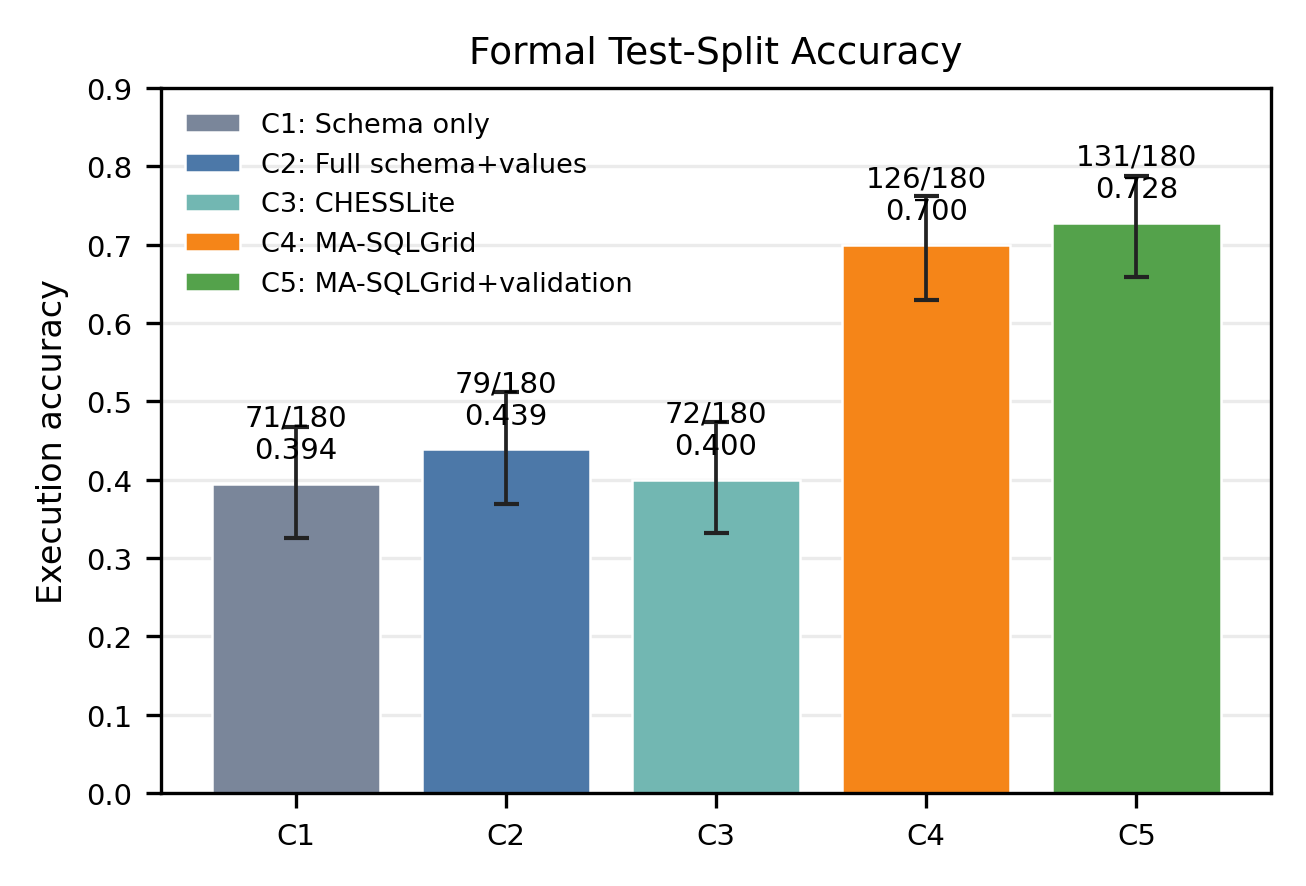
\includegraphics[width=11cm]{charts/fig_main_results.png}
\caption{Formal test-split execution accuracy by condition with item-level Wilson intervals over the 180 test questions.}
\label{fig:main-results}
\end{figure}

The answer-shape metric adds a second layer of interpretation. C1 reaches answer-shape accuracy of 0.3278, C2 reaches 0.3667, C3 reaches 0.5056, C4 reaches 0.8889, and C5 reaches 0.9722. The shape gain from C3 to C4 is substantial, which suggests that generic multi-stage prompting is not enough on its own. Shape inference matters most when it is paired with domain normalization. The validated condition then improves shape consistency again, which indicates that validation is not only rejecting invalid SQL but also preferring candidates whose result form matches the question.

Value-hint coverage is treated as an internal trace diagnostic rather than a headline metric: in the runner, a prediction with no inferred value hints receives a vacuous coverage value of 1.0, so this quantity is useful for auditing domain-context traces but not for ranking conditions. The more direct evidence for the contribution of value hints within C4 is the no-value-hint ablation, which reduces the number of correct predictions from 126 to 118; the C4--C2 comparison remains confounded by simultaneous differences in context scope and answer-shape guidance. The trace-level coverage audit helps interpret this point without changing the main metric: among the 180 held-out test questions, 170 produced at least one normalized value hint in the domain context, with 330 normalized hint instances and 111 unique rendered hints over 20 matched value columns. These numbers are not used to score predictions, but they show that the normalizer was active on most of the formal split rather than only on a small hand-picked subset.

\subsection{Evaluation-Convention Sensitivity}\label{evaluation-convention-sensitivity}

All 900 predictions were also re-scored under an order-insensitive metric and a combined order-insensitive, projection-tolerant metric. Relaxing order alone preserves the condition ranking: C2 increases from 0.4389 to 0.4778, and C4 increases from 0.7000 to 0.7444. After order has been relaxed, adding projection tolerance increases C2 from 0.4778 to 0.8722, whereas C4 remains at 0.7444. The strict C4--C2 difference is therefore highly sensitive to the evaluator's projection and ordering conventions. The strict metric remains operationally relevant to the stated answer contract, but the combined relaxed result prevents the strict difference from being interpreted as evidence that C4 retrieves the intended row content more effectively. Because the combined comparator also changes projection handling, it should not itself be treated as a pure measure of row-content retrieval. Table~\ref{tab:second-model} reports the corresponding values for both generators and shows the same reversal for \texttt{deepseek-chat}.

\subsection{Component Ablation}\label{sect:r3}

To examine the two prompt-side hint channels more directly, an addendum run removed one C4 channel at a time while preserving the same held-out test split, generator, temperature-zero decoding, and no-gold prediction contract. Removing value hints reduces the number of correct predictions from 126/180 to 118/180. Removing answer-shape hints reduces it to 77/180 and lowers the reported answer-shape accuracy to 0.4389. These one-at-a-time ablations provide numerical evidence that both hint channels contribute within the tested C4 configuration, with a larger reduction after removing answer-shape hints. They do not identify independent main effects or interactions between context scope, value hints, and shape guidance; doing so requires the missing factorial comparison.

\subsection{Second-Generator Validation and Consistency}\label{second-generator-validation}

The second-generator protocol described in Section~4 re-ran C2, C4, and C5 with \texttt{deepseek-chat} on the same 180 held-out test questions using byte-identical archived prompts and the same packaged evaluator. Table~\ref{tab:second-model} reports strict and relaxed metrics for both generators side by side.

\begin{table}[H]
\tablesize{\small}
\caption{Cross-model comparison on the 180-question test split under strict and relaxed metrics. The \texttt{deepseek-chat} rows use byte-identical prompts, temperature 0, and the same evaluator.}
\label{tab:second-model}
\centering
\begin{adjustbox}{max width=\textwidth}
\begin{tabular}{llrrr}
\toprule
\textbf{Generator} & \textbf{Condition} & \textbf{Strict (primary)} & \textbf{Order-insensitive} & \textbf{Order-insensitive + projection-tolerant} \\
\midrule
\texttt{gpt-5.4-mini} & C2 & 0.4389 (79/180) & 0.4778 & 0.8722 \\
\texttt{gpt-5.4-mini} & C4 & 0.7000 (126/180) & 0.7444 & 0.7444 \\
\texttt{gpt-5.4-mini} & C5 & 0.7278 (131/180) & 0.7722 & 0.8056 \\
\midrule
\texttt{deepseek-chat} & C2 & 0.3389 (61/180) & 0.3667 & 0.8500 \\
\texttt{deepseek-chat} & C4 & 0.7000 (126/180) & 0.7944 & 0.7944 \\
\texttt{deepseek-chat} & C5 & 0.7667 (138/180) & 0.8278 & 0.8278 \\
\bottomrule
\end{tabular}
\end{adjustbox}
\end{table}

Three numerical patterns recur for the second generator. First, the strict C4--C2 difference is larger on \texttt{deepseek-chat}: C4 exceeds C2 by 36.1 percentage points (0.3389 to 0.7000), compared with 26.1 percentage points (0.4389 to 0.7000) on \texttt{gpt-5.4-mini}. The C4 strict score is coincidentally identical for the two generators (126/180). Second, C5 exceeds C4 by 6.7 percentage points on \texttt{deepseek-chat} (0.7000 to 0.7667), compared with a statistically nonsignificant 2.8-percentage-point difference for the primary generator. Third, the reversal under the combined order-insensitive and projection-tolerant metric also recurs: C2 exceeds C4 for both generators (0.8500 versus 0.7944 on \texttt{deepseek-chat}; 0.8722 versus 0.7444 on \texttt{gpt-5.4-mini}). For \texttt{deepseek-chat}, adding projection tolerance after order relaxation does not further change C4 or C5. These results show that the sensitivity of the strict C4--C2 difference to answer-contract conventions is not confined to one generator. Condition-level paired tests for the \texttt{deepseek-chat} comparisons should be reported before the numerical differences are described as confirmed effect replications.

The second-generator run provides a separate within-endpoint resource comparison (Supplementary Table~S4). Provider-reported input counts on the direct endpoint are substantially closer to the rendered-prompt estimates than those on the original serving stack: C4 uses 509.3 input tokens per question, compared with 2011.6 for C2, a reduction of 74.7\%. This within-endpoint percentage should not be compared directly with the 23.4\% reduction on the original serving stack because the two endpoints use different token accounting and serving configurations. C5 uses about four times as many completion tokens as C4 (186.2 versus 46.6) and has approximately three times the mean latency (3014.2 versus 1054.0~ms), reflecting the cost of multi-candidate validation. C2 and C4 completed all 360 question-condition records without retries, whereas C5 required one retry for 2 of 180 records. The full run produced 540 question-condition records and consumed 576.3 thousand input tokens and 50.9 thousand output tokens, with zero final provider errors. The total number of API attempts, including retries and any repair calls, should be reported separately.

The companion consistency check measures run-to-run variation for the repeated \texttt{deepseek-chat} C4 and C5 conditions. Each condition was run three additional times at temperature 0, yielding 1,080 question-condition records. Per-run strict execution accuracy was 0.7056/0.6944/0.7000 for C4 and 0.7667/0.7667/0.7611 for C5, corresponding to a maximum spread of 1.1 percentage points. Exact SQL string agreement across all three runs was lower (82.2\% of questions for C4 and 77.2\% for C5), confirming that hosted endpoints can produce token-level variation even at temperature 0. Nevertheless, all three runs produced the same correct/incorrect verdict for 98.3\% of questions in both conditions. These results support run-level stability only for the repeated \texttt{deepseek-chat} C4 and C5 conditions; no repeated-run claim is made for the primary generator or the other conditions. The 898/900 first-attempt-call rate in the primary run documents API reliability rather than output stability.

The boundary of this validation should be stated as precisely as the result. The study now covers two generator families, one closed (\texttt{gpt-5.4-mini}) and one open-weight served through its provider endpoint (\texttt{deepseek-chat}); no third family was tested, and the cross-model comparison is at the aggregate level, with no per-question significance test across models. The C5 stage for the second generator is a specification-faithful reimplementation validated at 98.8\% selection agreement against the archive, not the original binary. Within those bounds, the principal condition differences have the same direction and larger numerical magnitudes for the second generator; condition-level paired significance tests remain necessary before describing these differences as confirmed effect replications.

\subsection{Asymmetric Asset-Row Scaling Diagnostic}\label{scale-robustness}

An asymmetric scaling diagnostic increased the asset table to 180 rows and added two distractor tables, after which C2, C4, and C5 were evaluated with \texttt{deepseek-chat} on the same 180 questions. C4 achieves a strict accuracy of 0.5944, compared with 0.3333 for C2, and C5 achieves 0.6500; provider-reported C2 input grows by 51\%, whereas C4 remains near 504 tokens per question. This experiment is not a symmetric database-scale or schema-generalization test because the distractor tables are included in the full-schema prompt but excluded by the compact builder's fixed eight-table catalog. Its main diagnostic value is that it exposes a \texttt{LIMIT 80} value-inventory failure. A scalable value index and a future stress test in which semantically confusable tables enter both candidate paths are therefore required before making scale-robustness claims \cite{talaei2024chess}. Full metrics are reported in Supplementary Section~S3.

\subsection{Error Analysis and Case Studies}\label{sect:r5}

The archived taxonomy (Supplementary Table~S6) shows that shape mismatch dominates C1--C3 but is no longer the primary residual failure for C4/C5. C4 has 34 wrong-denotation errors and 20 execution errors; C5 reduces execution errors from 20 to 5, while wrong-denotation errors increase from 34 to 44. Thus, validation improves executability but does not consistently reduce semantic errors. Recurrent residual failures include schedule-column naming errors rooted in schema-selection misses. Full trace diagnostics, tag-level results, the claim-to-evidence map, and the three SQL case studies are provided in Supplementary Tables~S5--S7 and Section~S2.

\subsection{Discussion}\label{sect:r6}

The main result is that the complete C4 configuration achieves higher strict execution accuracy than C1--C3 on this fixed database. C4 combines compact schema selection, domain-specific value normalization, and question-specific answer-shape guidance; the present comparison therefore establishes a configuration-level difference rather than the independent effect of compactness. This pattern is consistent with prior work on selective schema grounding and structured prompting \cite{lei2020reexamining,liu2022semantic,quamar2022natural,xie2022unifiedskg}. The one-at-a-time ablations further show numerical decreases when either shape hints or value hints are removed from C4, with a larger decrease after removing shape hints. However, these ablations do not establish an interaction between the two hint channels or show that the C3--C4 difference is caused specifically by value canonicalization. Together with the reversal under the combined relaxed metric, the evidence indicates that the tested C4 configuration is particularly effective at producing answers that conform to the benchmark's strict projection and ordering contract.

The validation layer requires a separate interpretation. For the primary generator, C5 exceeds C4 by 2.8 percentage points in strict accuracy, but this item-level difference is not statistically significant. The residual-error taxonomy shows that C5 reduces execution errors from 20 to 5 while increasing wrong-denotation errors from 34 to 44. Validation therefore improves executability and some aspects of answer-contract conformance, but it does not consistently reduce semantic errors. Its contribution should be interpreted as a bounded selection-and-repair effect rather than as a substitute for the prompt-side configuration \cite{wang2021executions,li2024select,huang2024survey}.

The observed runtime tradeoff is relevant within this benchmark. C4 has a slightly lower mean latency than C2 in the reported run, whereas C5 is slower because it generates and evaluates multiple candidates. C4 therefore provides the more favorable strict-accuracy/latency point estimate in this experiment. C5 has the highest strict-accuracy point estimate, but its increment over C4 is not statistically significant for the primary generator, and C2 has the highest score under the combined relaxed metric. These results do not support a general deployment recommendation or a claim of production readiness. Instead, they show that a bounded control loop can be evaluated efficiently when the schema and domain vocabulary are fixed \cite{wang2023macsql,pourreza2024chasesql}.

The broader implication is modest but useful. In this tightly scoped database, the compact contract-aware prompt outperforms a fuller prompt under the strict evaluator. This is relevant to power-grid maintenance tasks, where literal matching and answer-shape control are important, but it should not be read as a general rule that shorter prompts are intrinsically better. A validator over poorly grounded candidates cannot reliably recover missing domain evidence, while a grounded candidate set gives the selector more useful alternatives. The experiment therefore supports the tested sequence of schema selection, value normalization, shape control, generation, and reference-free selection on this benchmark; isolating compactness from contract guidance requires the missing factorial comparison.

\section{Conclusions and Limitations}\label{conclusion}

MA-SQLGrid shows that a lightweight multi-stage Text-to-SQL pipeline can improve strict contract-compliant accuracy on a fixed power-grid maintenance database. The complete C4 configuration, which combines compact schema and value context, domain normalization, and answer-shape guidance, achieves higher strict accuracy than the tested broader prompting baselines. C5 has a still higher strict point estimate, although its increment over C4 is not statistically significant for the primary generator. The same directions and the same evaluation-convention sensitivity are observed for a second generator, with larger numerical condition differences. Because the full-schema condition becomes stronger under the combined order-insensitive and projection-tolerant metric, the evidence is strongest for improved conformance to the benchmark's explicit answer contract rather than for an independently identified compactness effect or superior row-content retrieval.

The study is tied to one synthetic deterministic database, so its findings concern this benchmark rather than enterprise schemas generally \cite{zhong2020semantic,lei2024spider}. Run-to-run variation is bounded only for the second generator, and hosted model changes may affect exact reproduction despite the archived traces. The second-generator C5 stage is a specification-faithful reimplementation (98.8\% selection agreement), not the original binary. The row-scaling test asymmetrically stresses the full-schema condition and exposes a fixed-cap value-inventory failure. Most importantly, the present comparisons do not include the full $2\times2$ factorial needed to separate context scope from answer-shape hints (full versus compact context, each with and without identical shape hints). The no-shape and no-value ablations identify channels inside C4, but a future frozen run must add a full-schema-plus-shape condition before the compactness mechanism can be generalized independently of contract guidance. The validated condition adds latency and its original C5--C4 increment is not significant. The evidence is therefore strongest for the complete contract-aware pipeline on this benchmark, not for cross-database superiority of every component.

Future work should test the same design under schema drift and with generator families beyond the two evaluated here, replace the fixed-cap value inventory with a scalable value index and re-test at larger scales, repeat the evaluation on public benchmarks, expand the error analysis by query type, and evaluate whether compact grounding transfers to other infrastructure databases with similarly structured vocabularies.

% 可能要删掉或者写别的
% \acknowledgement{During the preparation of this work, the authors used OpenAI Codex (GPT-5-based) in order to assist with drafting, editing, code review, and reproducibility checks. After using this service, the authors reviewed and revised the relevant content and take full responsibility for the content of the published article. The hosted models evaluated in this study (\texttt{gpt-5.4-mini} and \texttt{deepseek-chat}) are experimental subjects rather than writing tools; all outputs are archived in the released artifact traces, and all reported numbers were computed from those artifacts.}

\funding{This research received no specific funding.}

\authorcontributions{The authors confirm their contributions to the paper as follows: conceptualization, methodology, software, and writing---original draft preparation, B.L.; validation, data curation, investigation, and writing---review and editing, C.S.; supervision, project administration, and writing---review and editing, Y.Y. All authors reviewed and approved the final version of the manuscript.}

\availabilityofdataandmaterials{The data and code supporting this study are openly available in the MA-SQLGrid repository at \url{https://github.com/gaoxingkele/ma-sqlgrid} (release v0.2.0). The release includes the frozen GridDB-Maintenance-v2 v0.1 dataset, the semantic evaluator and unit tests, condition prompts and context hashes, prediction and score records, raw API traces, repeated-run and scaling diagnostics, component-ablation outputs, and scripts that recompute the reported results. The context-builder and smoke-test modules included in release v0.2.0 reproduce the 180 archived formal-run prompts byte-for-byte. The original LLM client package and the v0.1 dataset-generation script are unavailable; the release instead provides a documented client-compatibility shim and archived dataset-provenance records. The released artifacts permit recomputation of the reported results, but the original dataset-generation process cannot be fully regenerated without the missing script.}

\ethicsapproval{Not applicable, as this study did not involve human or animal subjects.}

\conflictsofinterest{The authors declare no conflicts of interest.}

\supplementary{The following supplementary materials are available online at \linksupplementary{}: Section S1: verbatim prompt templates for the five experimental conditions, including the rendered compact domain context example and the C5 candidate-generation and bounded-repair templates; Section S2: per-question case SQL listings for the three case studies; Table S1: implementation details fixed in the reported MA-SQLGrid run; Table S2: dataset characterization for GridDB-Maintenance-v2 v0.1; Table S3: paired per-question comparisons on the test split; Table S4: measured resource consumption for the \texttt{deepseek-chat} second-generator run; Table S5: execution accuracy by question tag; Table S6: residual error taxonomy from the archived formal run; Table S7: claim-to-evidence map; Section S3: asymmetric asset-row scaling diagnostic, with Table S8 (full v0.1-versus-scaled metric comparison), Table S9 (token economics at scale), and the value-inventory artifact diagnosis.}

%=====================================
% References
%=====================================
\reftitle{References}
\begin{thebibliography}{10}

\bibitem{zhong2020semantic}
Zhong R, Yu T, Klein D.
\newblock Semantic evaluation for text-to-SQL with distilled test suites.
\newblock In: Proceedings of the 2020 Conference on Empirical Methods in
  Natural Language Processing (EMNLP); 2020 Nov 16--20; Online; 2020. Available
  from: \url{https://doi.org/10.18653/v1/2020.emnlp-main.29}.

\bibitem{lei2020reexamining}
Lei W, Wang W, Ma Z, Gan T, Lu W, Kan MY, et~al.
\newblock Re-examining the role of schema linking in text-to-SQL.
\newblock In: Proceedings of the 2020 Conference on Empirical Methods in
  Natural Language Processing (EMNLP); 2020 Nov 16--20; Online; 2020. Available
  from: \url{https://doi.org/10.18653/v1/2020.emnlp-main.564}.

\bibitem{liu2022semantic}
Liu A, Hu X, Li L, Wen L.
\newblock Semantic enhanced text-to-SQL parsing via iteratively learning schema
  linking graph.
\newblock In: Proceedings of the 28th ACM SIGKDD Conference on Knowledge
  Discovery and Data Mining; 2022 Aug 14--18; Washington, DC, USA; 2022.
  Available from: \url{https://doi.org/10.1145/3534678.3539294}.

\bibitem{quamar2022natural}
Quamar A, Efthymiou V, Lei C, Lei C.
\newblock Natural language interfaces to data.
\newblock Found Trends Databases. 2022;11(4):319-414.
\newblock Available from: \url{https://doi.org/10.1561/1900000078}.

\bibitem{gan2021robustness}
Gan Y, Chen X, Huang Q, Purver M, Woodward JR, Xie J, et~al.
\newblock Towards robustness of text-to-SQL models against synonym
  substitution.
\newblock In: Proceedings of the 59th Annual Meeting of the Association for
  Computational Linguistics (ACL); 2021 Aug 1--6; Online; 2021. Available from:
  \url{https://doi.org/10.18653/v1/2021.acl-long.195}.

\bibitem{liu2021awakening}
Liu Q, Yang D, Zhang J, Guo J, Zhou B, Lou JG.
\newblock Awakening latent grounding from pretrained language models for
  semantic parsing.
\newblock In: Findings of the Association for Computational Linguistics:
  ACL-IJCNLP 2021; 2021 Aug 1--6; Online; 2021. Available from:
  \url{https://doi.org/10.18653/v1/2021.findings-acl.100}.

\bibitem{chang2023prompt}
Chang S, Fosler-Lussier E.
\newblock How to prompt LLMs for text-to-SQL: a study in zero-shot,
  single-domain, and cross-domain settings [Preprint]; 2023.
\newblock Available from: \url{https://arxiv.org/abs/2305.11853}.
\newblock arXiv:2305.11853.

\bibitem{nan2023enhancing}
Nan L, Zhao Y, Zou W, Ri N, Tae J, Zhang E, et~al.
\newblock Enhancing text-to-SQL capabilities of large language models: a study
  on prompt design strategies.
\newblock In: Findings of the Association for Computational Linguistics: EMNLP
  2023; 2023 Dec 6--10; Singapore; 2023. Available from:
  \url{https://doi.org/10.18653/v1/2023.findings-emnlp.996}.

\bibitem{sun2023sqlprompt}
Sun R, Arik SO, Sinha R, Nakhost H, Dai H, Yin P, et~al.
\newblock SQLPrompt: in-context text-to-SQL with minimal labeled data
  [Preprint]; 2023.
\newblock Available from: \url{https://arxiv.org/abs/2311.02883}.
\newblock arXiv:2311.02883.

\bibitem{pourreza2023dinsql}
Pourreza M, Rafiei D.
\newblock DIN-SQL: decomposed in-context learning of text-to-SQL with
  self-correction [Preprint]; 2023.
\newblock Available from: \url{https://arxiv.org/abs/2304.11015}.
\newblock arXiv:2304.11015.

\bibitem{wang2023macsql}
Wang B, Ren C, Yang J, Liang X, Bai J, Chai L, et~al.
\newblock MAC-SQL: a multi-agent collaborative framework for text-to-SQL
  [Preprint]; 2023.
\newblock Available from: \url{https://arxiv.org/abs/2312.11242}.
\newblock arXiv:2312.11242.

\bibitem{talaei2024chess}
Talaei S, Pourreza M, Chang YC, Mirhoseini A, Saberi A.
\newblock CHESS: contextual harnessing for efficient SQL synthesis [Preprint];
  2024.
\newblock Available from: \url{https://arxiv.org/abs/2405.16755}.
\newblock arXiv:2405.16755.

\bibitem{liu2024survey}
Liu X, Shen S, Li B, Ma P, Runzhi J, Zhang Y, et~al.
\newblock A survey of text-to-SQL in the era of LLMs: where are we, and where
  are we going? [Preprint]; 2024.
\newblock Available from: \url{https://arxiv.org/abs/2408.05109}.
\newblock arXiv:2408.05109.

\bibitem{katsogiannismeimarakis2023survey}
Katsogiannis-Meimarakis G, Koutrika G.
\newblock A survey on deep learning approaches for text-to-SQL.
\newblock VLDB J. 2023;32(4):905-36.
\newblock Available from: \url{https://doi.org/10.1007/s00778-022-00776-8}.

\bibitem{huang2024survey}
Huang X, Ruan W, Huang W, Jin G, Dong Y, Wu C, et~al.
\newblock A survey of safety and trustworthiness of large language models
  through the lens of verification and validation.
\newblock Artif Intell Rev. 2024;57(7):175.
\newblock Available from: \url{https://doi.org/10.1007/s10462-024-10824-0}.

\bibitem{wu2022chains}
Wu T, Terry M, Cai CJ.
\newblock AI chains: transparent and controllable human-AI interaction by
  chaining large language model prompts.
\newblock In: Proceedings of the 2022 CHI Conference on Human Factors in
  Computing Systems; 2022 Apr 29--May 5; New Orleans, LA, USA; 2022. Available
  from: \url{https://doi.org/10.1145/3491102.3517582}.

\bibitem{xie2022unifiedskg}
Xie T, Wu C, Shi P, Zhong R, Scholak T, Yasunaga M, et~al.
\newblock UnifiedSKG: unifying and multi-tasking structured knowledge grounding
  with text-to-text language models.
\newblock In: Proceedings of the 2022 Conference on Empirical Methods in
  Natural Language Processing (EMNLP); 2022 Dec 7--11; Abu Dhabi, United Arab
  Emirates; 2022. Available from:
  \url{https://doi.org/10.18653/v1/2022.emnlp-main.39}.

\bibitem{li2024select}
Li Z, Xie T.
\newblock Using LLM to select the right SQL query from candidates [Preprint];
  2024.
\newblock Available from: \url{https://arxiv.org/abs/2401.02115}.
\newblock arXiv:2401.02115.

\bibitem{lee2021kaggledbqa}
Lee CH, Polozov O, Richardson M.
\newblock KaggleDBQA: realistic evaluation of text-to-SQL parsers.
\newblock In: Proceedings of the 59th Annual Meeting of the Association for
  Computational Linguistics (ACL); 2021 Aug 1--6; Online; 2021. Available from:
  \url{https://doi.org/10.18653/v1/2021.acl-long.176}.

\bibitem{lei2024spider}
Lei F, Chen J, Ye Y, Cao R, Shin D, Su H, et~al.
\newblock Spider 2.0: evaluating language models on real-world enterprise
  text-to-SQL workflows [Preprint]; 2024.
\newblock Available from: \url{https://arxiv.org/abs/2411.07763}.
\newblock arXiv:2411.07763.

\bibitem{herzig2020tapas}
Herzig J, Nowak PK, Muller T, Piccinno F, Eisenschlos JM.
\newblock TaPas: weakly supervised table parsing via pre-training.
\newblock In: Proceedings of the 58th Annual Meeting of the Association for
  Computational Linguistics (ACL); 2020 Jul 5--10; Online; 2020. Available
  from: \url{https://doi.org/10.18653/v1/2020.acl-main.398}.

\bibitem{chen2023large}
Chen W.
\newblock Large language models are few(1)-shot table reasoners.
\newblock In: Findings of the Association for Computational Linguistics: EACL
  2023; 2023 May 2--6; Dubrovnik, Croatia; 2023. Available from:
  \url{https://doi.org/10.18653/v1/2023.findings-eacl.83}.

\bibitem{zhang2024structure}
Zhang Q, Chen H, Dong J, Chen S, Huang F, Huang X.
\newblock Structure guided large language model for SQL generation [Preprint];
  2024.
\newblock Available from: \url{https://arxiv.org/abs/2402.13284}.
\newblock arXiv:2402.13284.

\bibitem{liu2023divide}
Liu X, Tan Z.
\newblock Divide and prompt: chain of thought prompting for text-to-SQL
  [Preprint]; 2023.
\newblock Available from: \url{https://arxiv.org/abs/2304.11556}.
\newblock arXiv:2304.11556.

\bibitem{arora2023adapt}
Arora A, Bhaisaheb S, Nigam H, Patwardhan M, Vig L, Shroff G.
\newblock Adapt and decompose: efficient generalization of text-to-SQL via
  domain adapted least-to-most prompting [Preprint]; 2023.
\newblock Available from: \url{https://arxiv.org/abs/2308.02582}.
\newblock arXiv:2308.02582.

\bibitem{xie2024decomposition}
Xie Y, Jin X, Xie T, Matrixmxlin M, Chen L, Yu C, et~al.
\newblock Decomposition for enhancing attention: improving LLM-based
  text-to-SQL through workflow paradigm.
\newblock In: Findings of the Association for Computational Linguistics: ACL
  2024; 2024 Aug 11--16; Bangkok, Thailand; 2024. Available from:
  \url{https://doi.org/10.18653/v1/2024.findings-acl.641}.

\bibitem{xie2024magsql}
Xie W, Wu G, Zhou B.
\newblock MAG-SQL: multi-agent generative approach with soft schema linking and
  iterative sub-SQL refinement for text-to-SQL [Preprint]; 2024.
\newblock Available from: \url{https://arxiv.org/abs/2408.07930}.
\newblock arXiv:2408.07930.

\bibitem{cen2025sqlfixagent}
Cen J, Liu J, Li Z, Wang J.
\newblock SQLFixAgent: towards semantic-accurate text-to-SQL parsing via
  consistency-enhanced multi-agent collaboration.
\newblock In: Proceedings of the 39th AAAI Conference on Artificial
  Intelligence; 2025 Feb 25--Mar 4; Philadelphia, PA, USA; 2025. Available
  from: \url{https://doi.org/10.1609/aaai.v39i1.31979}.

\bibitem{guo2023evaluating}
Guo Z, Jin R, LIU C, Huang Y, Shi D, Supryadi, et~al.
\newblock Evaluating large language models: a comprehensive survey [Preprint];
  2023.
\newblock Available from: \url{https://arxiv.org/abs/2310.19736}.
\newblock arXiv:2310.19736.

\bibitem{wang2021executions}
Wang B, Lapata M, Titov I.
\newblock Learning from executions for semantic parsing.
\newblock In: Proceedings of the 2021 Conference of the North American Chapter
  of the Association for Computational Linguistics: Human Language Technologies
  (NAACL-HLT); 2021 Jun 6--11; Online; 2021. Available from:
  \url{https://doi.org/10.18653/v1/2021.naacl-main.219}.

\bibitem{chen2023texttosql}
Chen Z, Chen S, White M, Mooney RJ, Payani A, Srinivasa J, et~al.
\newblock Text-to-SQL error correction with language models of code.
\newblock In: Proceedings of the 61st Annual Meeting of the Association for
  Computational Linguistics (Short Papers); 2023 Jul 9--14; Toronto, ON,
  Canada; 2023. Available from:
  \url{https://doi.org/10.18653/v1/2023.acl-short.117}.

\bibitem{beyer2022verification}
Beyer D, Dangl M, Dietsch D, Heizmann M, Lemberger TR, Tautschnig M.
\newblock Verification witnesses.
\newblock ACM Trans Softw Eng Methodol. 2022;31(4):1-69.
\newblock Available from: \url{https://doi.org/10.1145/3477579}.

\bibitem{pauwels2024validation}
Pauwels P, van~den Bersselaar E, Verhelst L.
\newblock Validation of technical requirements for a BIM model using semantic
  web technologies.
\newblock Adv Eng Inform. 2024;60:102426.
\newblock Available from: \url{https://doi.org/10.1016/j.aei.2024.102426}.

\bibitem{zhai2025excot}
Zhai B, Xu C, He Y, Yao Z.
\newblock ExCoT: optimizing reasoning for text-to-SQL with execution feedback
  [Preprint]; 2025.
\newblock Available from: \url{https://arxiv.org/abs/2503.19988}.
\newblock arXiv:2503.19988.

\bibitem{pourreza2024chasesql}
Pourreza M, Li H, Sun R, Chung Y, Talaei S, Kakkar GT, et~al.
\newblock CHASE-SQL: multi-path reasoning and preference optimized candidate
  selection in text-to-SQL [Preprint]; 2024.
\newblock Available from: \url{https://arxiv.org/abs/2410.01943}.
\newblock arXiv:2410.01943.

\bibitem{soliman2026coret}
Soliman H, Gupta V, Roth D, Gurevych I.
\newblock CORE-T: COherent REtrieval of tables for text-to-SQL [Preprint];
  2026.
\newblock Available from: \url{https://arxiv.org/abs/2601.13111}.
\newblock arXiv:2601.13111.

\bibitem{ganesan2025unjoin}
Ganesan P, Jha RA, Roth D, Gupta V.
\newblock UNJOIN: enhancing multi-table text-to-SQL generation via schema
  simplification [Preprint]; 2025.
\newblock Available from: \url{https://arxiv.org/abs/2505.18122}.
\newblock arXiv:2505.18122.

\bibitem{yang2025marssql}
Yang H, Zhang J, He Z, Zhou A, Fung YR.
\newblock MARS-SQL: a multi-agent reinforcement learning framework for
  text-to-SQL [Preprint]; 2025.
\newblock Available from: \url{https://arxiv.org/abs/2511.01008}.
\newblock arXiv:2511.01008.

\bibitem{li2024seasql}
Li C, Shao Y, Li Y, Liu Z.
\newblock SEA-SQL: semantic-enhanced text-to-SQL with adaptive refinement
  [Preprint]; 2024.
\newblock Available from: \url{https://arxiv.org/abs/2408.04919}.
\newblock arXiv:2408.04919.

\bibitem{luo2026siriussql}
Luo L, Xie H, Shen S, Ma Z, Ling R, Xu H, et~al.
\newblock SIRIUS-SQL: anchoring multi-candidate text-to-SQL in execution
  feedback [Preprint]; 2026.
\newblock Available from: \url{https://arxiv.org/abs/2606.01246}.
\newblock arXiv:2606.01246.

\bibitem{tremante2026spotit}
Tremante A, He Y, Klopfenstein R, Wang Y, Narodytska N, Wu H.
\newblock SpotIt+: verification-based text-to-SQL evaluation with database
  constraints [Preprint]; 2026.
\newblock Available from: \url{https://arxiv.org/abs/2603.04334}.
\newblock arXiv:2603.04334.

\bibitem{zhou2026sqlstructeval}
Zhou Y, Zhang F, Guo Z, Chen Y, Zhang H, Nakov P, et~al.
\newblock SQLStructEval: structural evaluation of LLM text-to-SQL generation
  [Preprint]; 2026.
\newblock Available from: \url{https://arxiv.org/abs/2604.06736}.
\newblock arXiv:2604.06736.

\bibitem{arif2026agentagnostic}
Arif TJ, Singh K.
\newblock Agent-agnostic evaluation of SQL accuracy in production text-to-SQL
  systems [Preprint]; 2026.
\newblock Available from: \url{https://arxiv.org/abs/2604.28049}.
\newblock arXiv:2604.28049.

\bibitem{borovcak2026evaluating}
Borov{\v{c}}ak K, Bagi{\'{c}}~Babac M, Mornar V.
\newblock Evaluating open-source LLM agents for SQL generation and structured
  analytics on relational databases.
\newblock Comput Mater Contin. 2026;88(2):80.
\newblock Available from: \url{https://doi.org/10.32604/cmc.2026.078330}.

\bibitem{lin2020bridging}
Lin X, Socher R, Xiong C.
\newblock Bridging textual and tabular data for cross-domain text-to-SQL
  semantic parsing.
\newblock In: Findings of the Association for Computational Linguistics: EMNLP
  2020; 2020 Nov 16--20; Online; 2020. Available from:
  \url{https://doi.org/10.18653/v1/2020.findings-emnlp.438}.

\bibitem{brunner2020valuenet}
Brunner U, Stockinger K.
\newblock ValueNet: a natural language-to-SQL system that learns from database
  information [Preprint]; 2020.
\newblock Available from: \url{https://arxiv.org/abs/2006.00888}.
\newblock arXiv:2006.00888.

\end{thebibliography}


\end{document}
